%Preliminary Results Appendix
%Include in main doc using \input{file}
\section{Proof of Concept and Testing}
\counterwithin{figure}{section}
\begin{lstlisting}[language=C,caption={ESC Driver Script},label={lst:Driver_Script}]

#include<Servo.h>

//Define Constants

Servo esc;
const int MotorPin = 9;
const int Var_Resistor = A0;
int Resistor_Value = 0;
int time_value = 0;

void setup() {

//begin serial monitor & baud rate
Serial.begin(9600)

//set up motor connection
esc.attach(MotorPin);  

//Enable Variable Resistor Input
pinMode(Var_Resistor,INPUT); 

}

void loop() {

//Read the resistor value 
Resistor_Value=analogRead(Var_Resistor);

//Var_Resistor will be between 1-1024
// need to convert to 1060-1860
//1060-1860 is a range of 800, 800/1023=0.78201

//Conversion into req'd pulse width range
time_value=(Resistor_Value*0.78201)+1060;

//write the time signal to the servo motor
esc.writeMicroseconds(time_value);
Serial.println(time_value);


}

\end{lstlisting}

\newpage

\begin{figure}
	\centering
	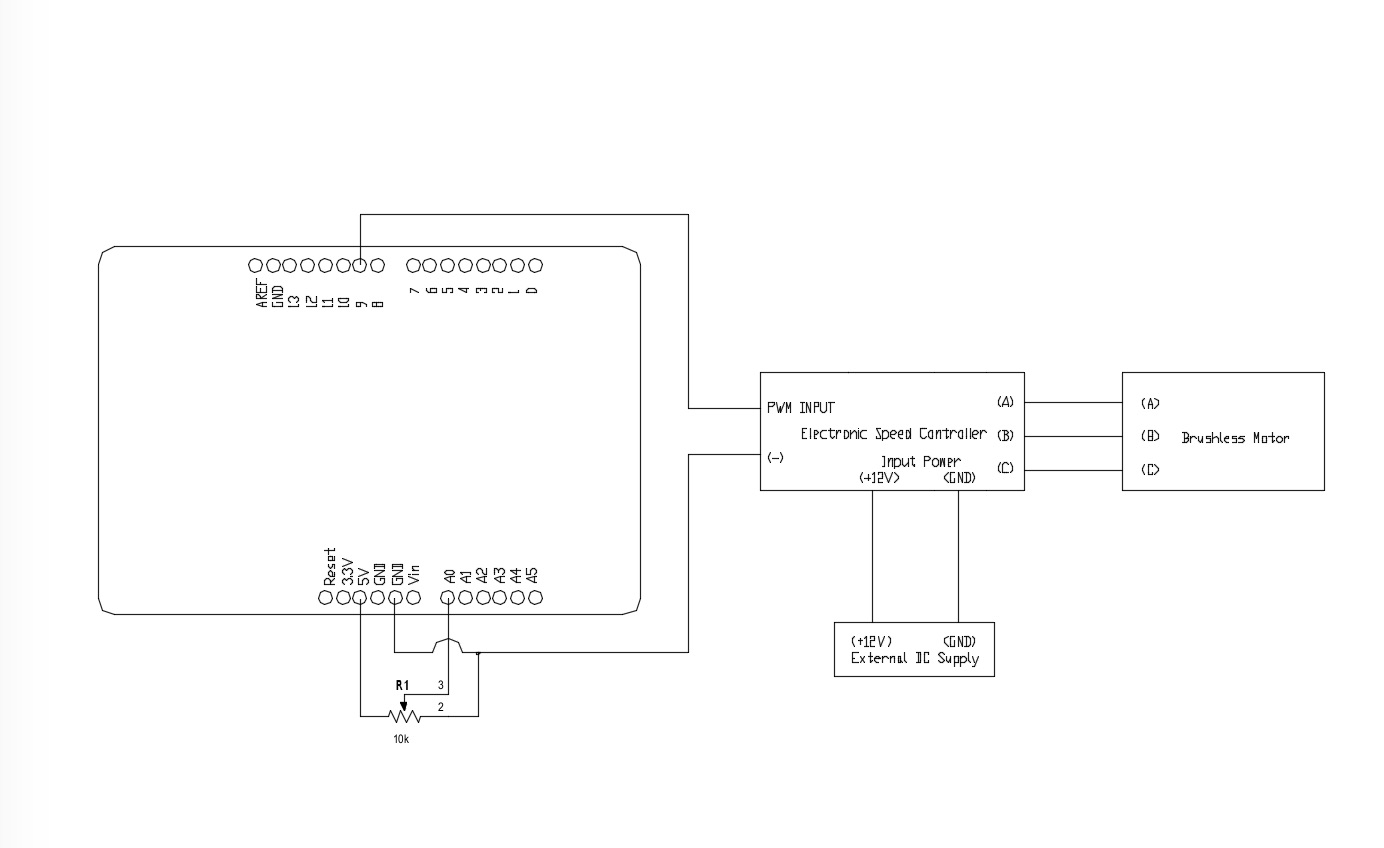
\includegraphics[width=1\textwidth]{Motor_Driving_Schematic.jpg}
	\caption{Motor Driver Circuit POC Schematic}
	\label{fig:Motor_Drive_Schem}
\end{figure}

\begin{figure}
	\centering
	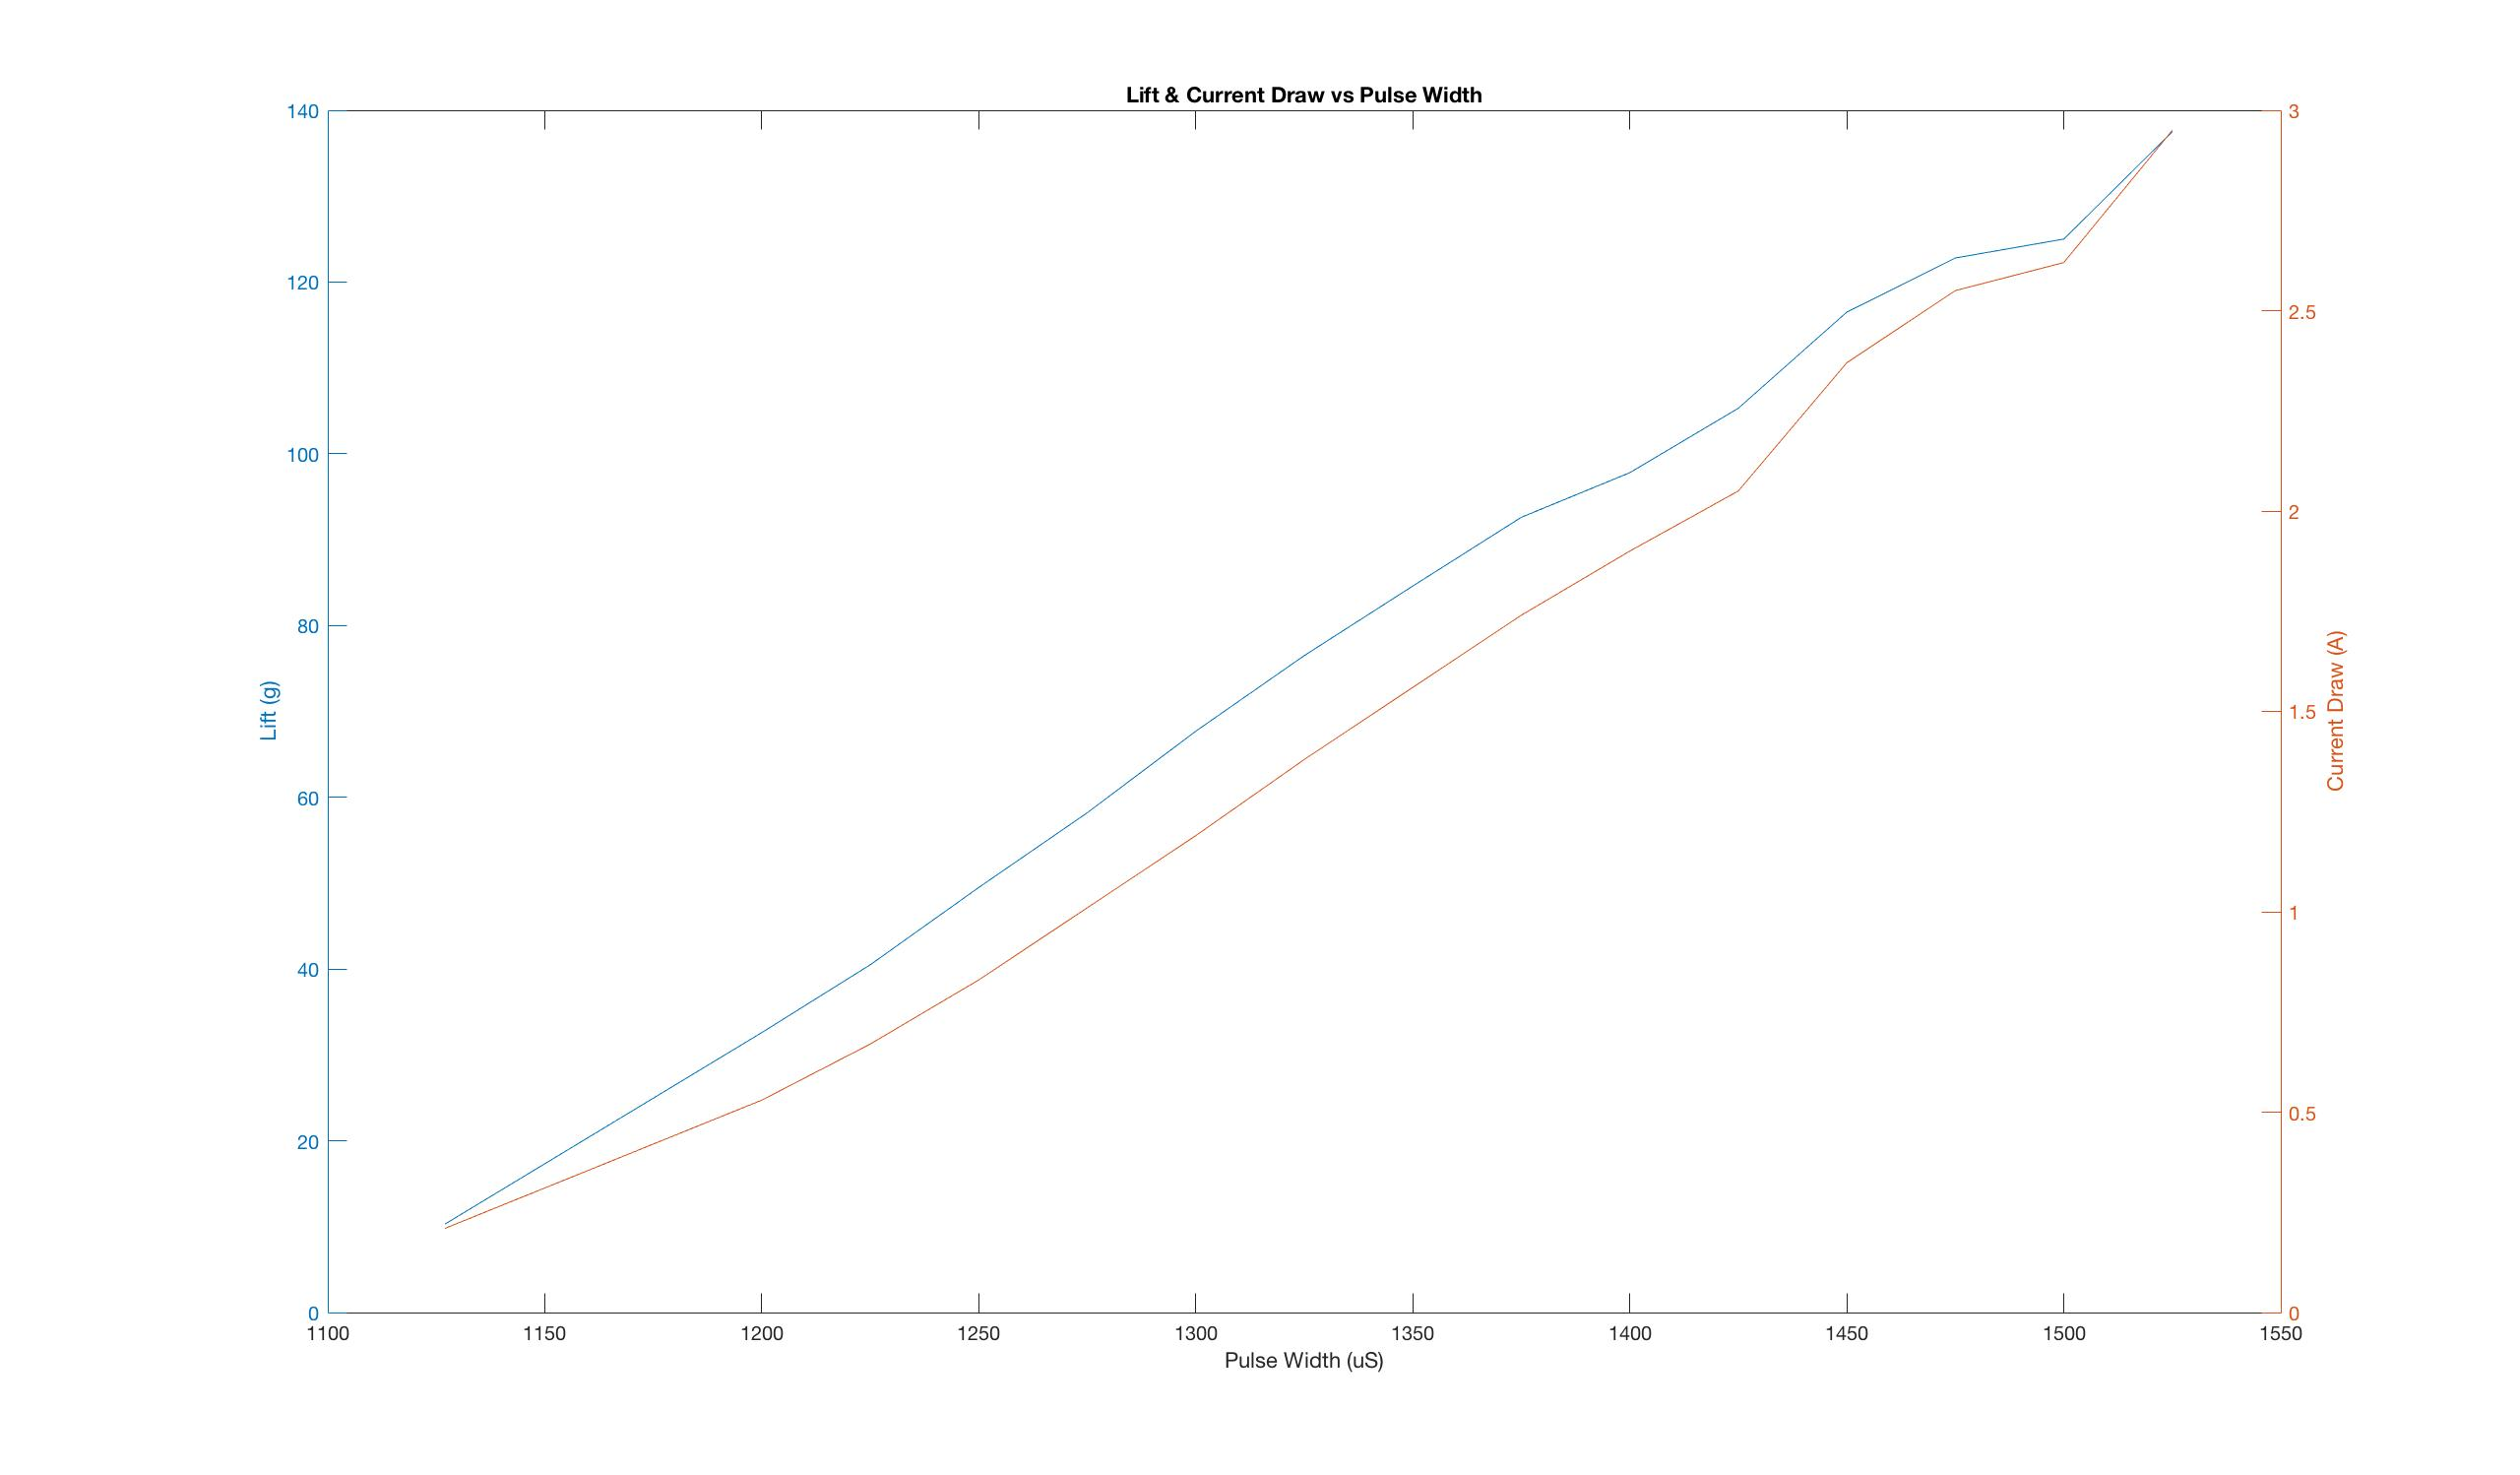
\includegraphics[width=1\textwidth]{Motor_Characterization.jpg}
	\caption{Motor Characterization Testing}
	\label{fig:Motor_Char}
\end{figure}


